% Copyright 2004 by Till Tantau <tantau@users.sourceforge.net>.
%
% In principle, this file can be redistributed and/or modified under
% the terms of the GNU Public License, version 2.
%
% However, this file is supposed to be a template to be modified
% for your own needs. For this reason, if you use this file as a
% template and not specifically distribute it as part of a another
% package/program, I grant the extra permission to freely copy and
% modify this file as you see fit and even to delete this copyright
% notice. 

\documentclass{beamer}

% There are many different themes available for Beamer. A comprehensive
% list with examples is given here:
% http://deic.uab.es/~iblanes/beamer_gallery/index_by_theme.html
% You can uncomment the themes below if you would like to use a different
% one:
% \usetheme{AnnArbor}
% \usetheme{Antibes}
% \usetheme{Bergen}
% \usetheme{Berkeley}
% \usetheme{Berlin}
% \usetheme{Boadilla}
% \usetheme{boxes}
% \usetheme{CambridgeUS}
% \usetheme{Copenhagen}
% \usetheme{Darmstadt}
% \usetheme{default}
% \usetheme{Frankfurt}
% \usetheme{Goettingen}
% \usetheme{Hannover}
% \usetheme{Ilmenau}
% \usetheme{JuanLesPins}
\usetheme{Luebeck}
% \usetheme{Madrid}
% \usetheme{Malmoe}
% \usetheme{Marburg}
% \usetheme{Montpellier}
% \usetheme{PaloAlto}
% \usetheme{Pittsburgh}
% \usetheme{Rochester}
% \usetheme{Singapore}
% \usetheme{Szeged}
% \usetheme{Warsaw}

% \usecolortheme{seahorse}
% \usecolortheme{seagull}
% \usecolortheme{albatross}
% \usecolortheme{beaver}
% \usecolortheme{beetle}
\usecolortheme{crane}
% \usecolortheme{dolphin}
% \usecolortheme{dove}
% \usecolortheme{fly}
% \usecolortheme{lily}
% \usecolortheme{monarca}
% \usecolortheme{orchid}
% \usecolortheme{rose}
% \usecolortheme{seagull}
% \usecolortheme{seahorse}
% \usecolortheme{spruce}
% \usecolortheme{whale}
% \usecolortheme{wolverine}

\title[Analysis and Coordination of Mixed-criticality CPSs]{Analysis and Coordination of Mixed-criticality Cyber-physical Systems}

% A subtitle is optional and this may be deleted
% \subtitle{Initial Registration Assessment}

\author{Simon Maurer}
% - Give the names in the same order as the appear in the paper.
% - Use the \inst{?} command only if the authors have different
%   affiliation.

\institute % (optional, but mostly needed)
{
  % \inst{1}%
  % Department of Computer Science\\
  % University of Somewhere
  % \and
  % \inst{2}%
    School of Computer Science\\
    University of Hertfordshire\\
    Hatfield, United Kingdom}
% - Use the \inst command only if there are several affiliations.
% - Keep it simple, no one is interested in your street address.

\date{January 2018}
% - Either use conference name or its abbreviation.
% - Not really informative to the audience, more for people (including
%   yourself) who are reading the slides online

\subject{Theoretical Computer Science}
% This is only inserted into the PDF information catalog. Can be left
% out. 
\setbeamertemplate{navigation symbols}{%
    \usebeamerfont{footline}%
    \usebeamercolor[fg]{footline}%
    \hspace{1em}%
    \insertframenumber
}

% Let's get started
\begin{document}

{
\setbeamertemplate{navigation symbols}{}
\begin{frame}[plain]
    \titlepage
    \addtocounter{framenumber}{-1}
\end{frame}
}

% Section and subsections will appear in the presentation overview
% and table of contents.


%%%%%%%%%%%%%%%%%%%%%%%%%%%%%%%%%%%%%%%%%%%%%%%%%%%%%%%%%%%%%%%%%%%%%%%%%%%%%%%%%%%%%%
% \section{Introduction}
\begin{frame}{Analysis and Coordination of Mixed-criticality CPSs}{Problem Description and Contributions}
        \centering
    \begin{overlayarea}{7cm}{7cm}
        \only<1>{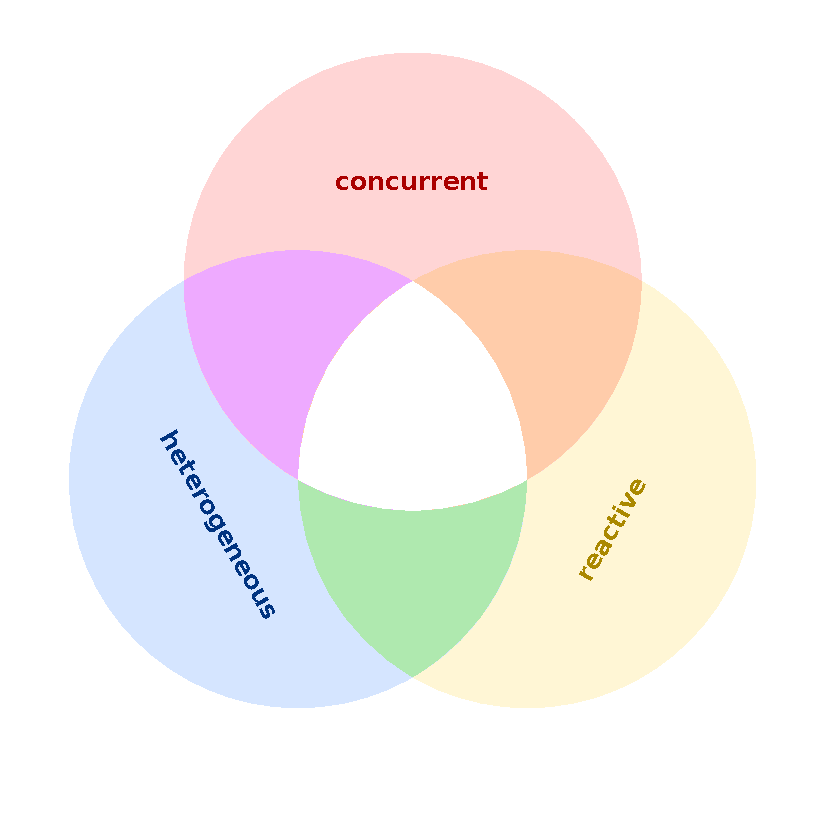
\includegraphics[width=7cm]{fig/trinity1.pdf}}
        \only<2>{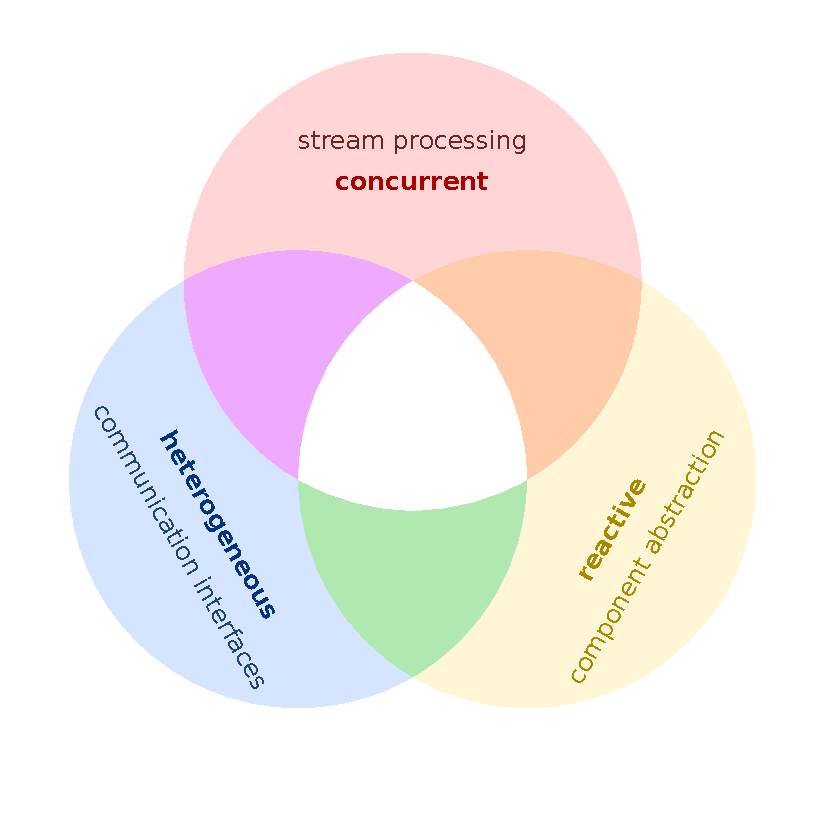
\includegraphics[width=7cm]{fig/trinity2.pdf}}
        \only<3>{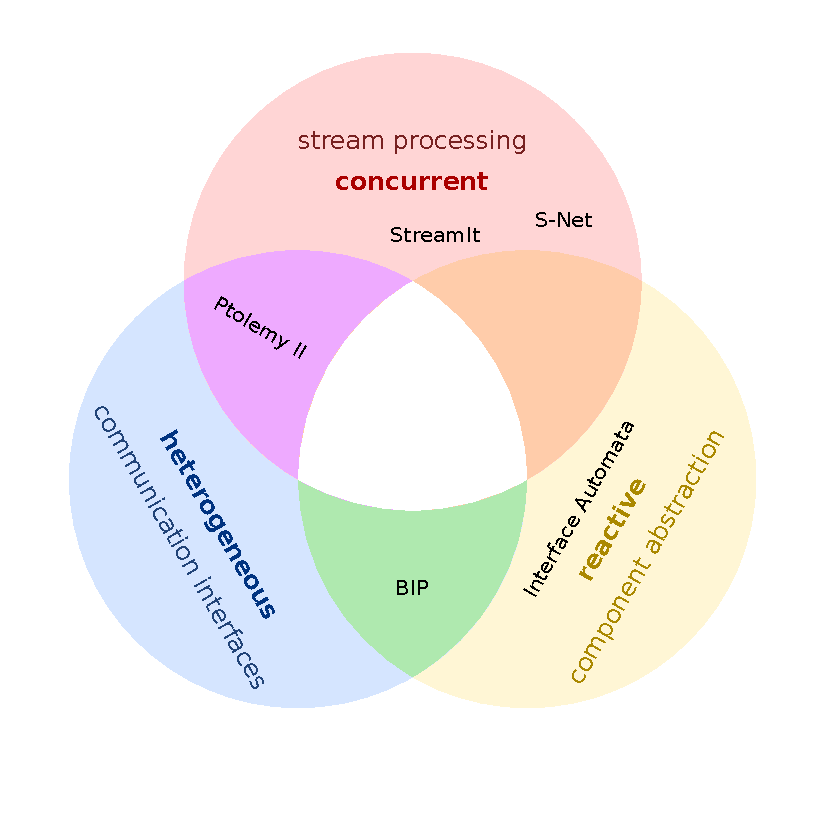
\includegraphics[width=7cm]{fig/trinity3.pdf}}
        \only<4>{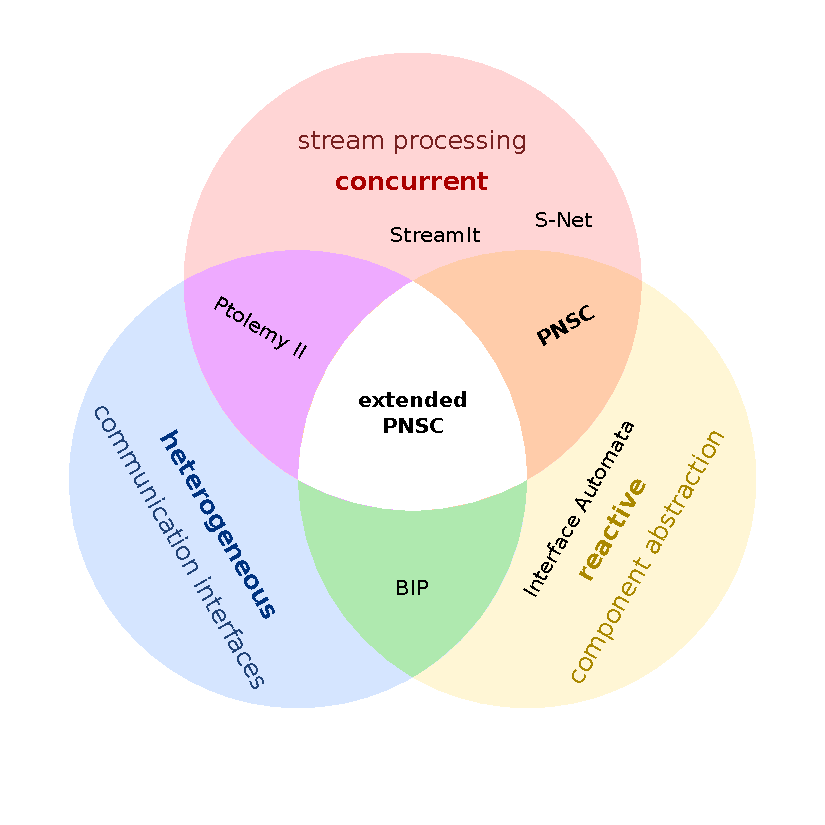
\includegraphics[width=7cm]{fig/trinity4.pdf}}
        \only<5>{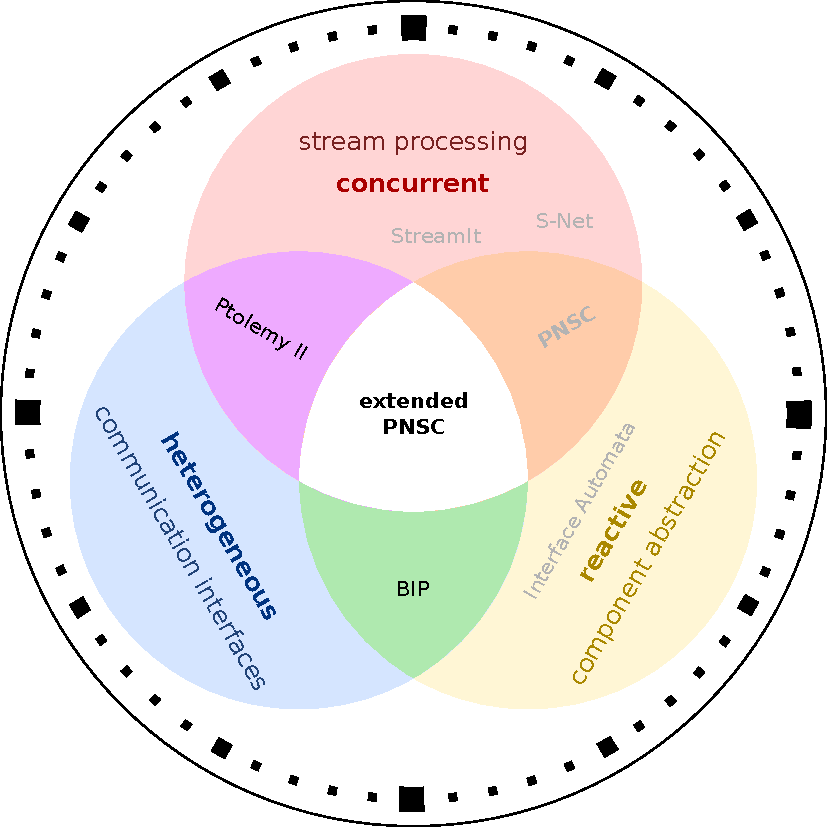
\includegraphics[width=7cm]{fig/trinity5.pdf}}
    \end{overlayarea}
\end{frame}
\begin{frame}{Interfaces for Strongly Coupled Reactive Components}{Research Question}
    \begin{block}{Question}
        What are suitable interfaces for reactive components with strong coupling to ensure correct behaviour of a system of such components assembled in a network?
    \end{block}
    \begin{itemize}
        \item support of complex components without loss of analysability
        \item detection of local and global permanent blocking situations
        \item composition of simple components into complex ones
    \end{itemize}
    \begin{exampleblock}{Answer}
        The Process Network with Syncronous Communication (PNSC) model and Synchronous Interface Automata (SIAs).
    \end{exampleblock}
\end{frame}
\begin{frame}{Interfaces for Mixed-criticality Components}{Research Question}
    \begin{block}{Question}
        What are suitable interfaces for CPSs to integrate subsystems with different criticality levels?
    \end{block}
    \begin{itemize}
        \item support of different communication schemes
        \item allow interaction while preventing unwanted interference
        \item fine-grained control on communication coupling
    \end{itemize}
    \begin{exampleblock}{Answer}
        The extension of the PNSC model with Cross-criticality Interfaces (CCIs) and rate control.
    \end{exampleblock}
\end{frame}
\begin{frame}{A Coordination Language for Reactive Components}{Research Question}
    \begin{block}{Question}
        What are the implications of reactive components on an exogenous coordination language?
    \end{block}
    \begin{itemize}
        \item structured programming for CPSs
        \item hierarchical construction of networks
    \end{itemize}
    \begin{exampleblock}{Answer}
        Using network operators to describe bidirectional communication.
    \end{exampleblock}
\end{frame}

% All of the following is optional and typically not needed. 
% \appendix

% \begin{frame}[allowframebreaks]
%     \frametitle<presentation>{For Further Reading}

%     \bibliography{../paper.bib}
%     % \bibliographystyle{IEEEtran}
%     \bibliographystyle{apalike}
% \end{frame}

\end{document}
